\bookchapter{Глава 37. Парадигмальная революция — от «писать код» к «командовать ИИ, который пишет код»}

\chapterintro{Поздравляем: открывая эту книгу, вы стоите в самом центре революции профессиональной парадигмы. Её отправная точка — фраза, которую один программист опубликовал в соцсетях в 2025 году. Звучит немного драматично? Но факты именно таковы.}

\booksection{Рождение Vibe Coding: движение, начавшееся с одной фразы}

В феврале 2025 года Andrej Karpathy — запомните это имя, вы ещё не раз его встретите — опубликовал в соцсетях твит, который потом цитировали бесконечно: «Есть новый способ программирования — Vibe Coding: вы полностью отдаётесь настроению (vibes), игнорируете детали кода и поручаете всё ИИ. Что видите — о том и говорите, копируете и вставляете, лишь бы в целом работало».

Это мимоходом брошенное высказывание на самом деле точно назвало уже тихо свершившийся парадигмальный сдвиг: человек больше не пишет код построчно — он описывает намерение на естественном языке, а реализацию завершает ИИ. Формулировка Karpathy звучит слегка иронично, но за ней глубокое наблюдение: когда способность ИИ генерировать код переходит определённый порог, узким местом программирования становится уже не «смогу ли я написать эту строку», а «насколько ясно я сам понимаю, что хочу сделать».

\begin{tcbinfo}{Совет: что такое Vibe?}
Vibe дословно — «атмосфера, настроение». Vibe Coding — это «управлять ИИ-программированием по настрою»: вы описываете, что хотите, а реализация — забота ИИ. Запомните это слово: оно — «свидетельство о рождении» всей революции.

\end{tcbinfo}

С того момента смысл слова «кодирование» начал раздваиваться: традиционное кодирование — это перевод замысла в синтаксис; новое кодирование — перевод намерения в инструкции. Первое испытывает пальцы, второе — голову.

Слово Vibe Coding быстро из шутки превратилось в серьёзное инженерное понятие. К середине 2026 года из мема в соцсетях оно выросло в целостную методологию — охватывающую весь путь от выражения требований и управления контекстом до итеративной проверки и контроля качества. Люди также осознали: «действовать по настрою» — лишь стадия новичка; по-настоящему эффективное программирование с ИИ требует системного способа мышления. А именно этот способ мышления и даёт вам эта книга.

\booksection{Ситуация в 2026 году: эра Agentic Engineering}

К августу 2026 года в ИИ-программировании уже произошло несколько важных смен парадигм. Vibe Coding была первой искрой, но быстро выяснилось: если просто «по настрою» болтать с ИИ, качество кода крайне нестабильно — то восторг, то провал. И парадигма стала эволюционировать: от простого диалогового программирования к структурированной инженерии агентов.

Снова Karpathy: в начале 2026 года он предложил понятие Agentic Engineering. В отличие от Vibe Coding с её «сказал — сгенерировано», Agentic Engineering подчёркивает: дайте ИИ цель, и пусть он самостоятельно планирует шаги, вызывает инструменты, проверяет результаты и итеративно исправляется. ИИ перестаёт быть просто генератором кода и становится агентом (Agent) — сущностью, способной воспринимать среду, принимать решения и выполнять действия.

Этот сдвиг принёс три ключевых изменения:

\begin{enumerate}
  \item Изменился режим взаимодействия: от «вопрос — ответ» к «поставил цель и делегировал полномочия».
  \item Изменился результат работы: от «куска кода» к «целостному проекту».
  \item Изменилась роль человека: от «построчной ревизии кода» к «определению границ и приёмке результата».
\end{enumerate}

Цифры не лгут: в Cursor 3, вышедшем в апреле 2026 года, доля использования режима Agent впервые превысила режим автодополнения Tab — разработчики массово перешли на новый способ работы; а Claude Code, нативный терминальный ИИ-инструмент для программирования, к середине 2026 года достиг годового дохода в 2,5 млрд долларов США (в годовом исчислении). График трендов ниже позволит вам наглядно ощутить момент этого пересечения:

\begin{center}
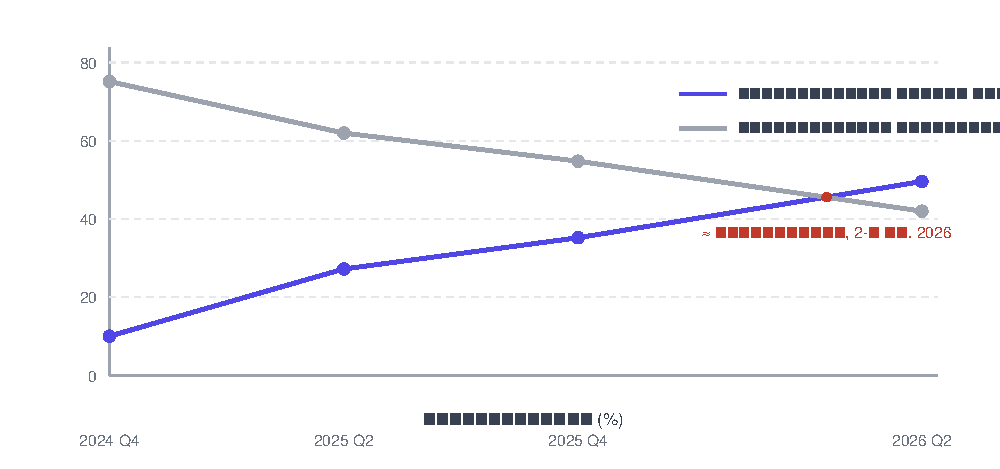
\includegraphics[width=0.92\linewidth]{figures/fig-di-san-shi-qi-zhang-1}
\\[2pt]\small Рисунок 1: тренд изменения долей режимов взаимодействия в ИИ-программировании (оценка на основе отраслевых исследований; во 2-м квартале 2026 года режим Agent обогнал автодополнение Tab)
\end{center}

Но скажем прямо: изменения инструментов и моделей — лишь внешняя сторона. Работаете ли вы в Cursor или Claude Code, стоит ли в основе GPT-5 или Claude 4.5 — успешные практики ИИ-программирования следуют одной и той же базовой методологии. Именно ей эта книга и учит.

\booksection{Ключевой сдвиг в сознании: от Coder к Conductor}

Классическое обучение программированию готовит вас стать Coder'ом — понимать синтаксис, запоминать API, отлаживать логические ошибки. В эпоху ИИ-программирования эта роль переопределяется. Вам больше не нужно своими руками писать каждую строку кода, но нужно стать «командиром» (Conductor): определить поле боя, установить правила, распределить задачи, принять результат.

Суть перехода не в том, «умеете ли вы писать код», а в том, «умеете ли вы ясно понять, что нужно сделать». Хороший командир не обязательно лучший солдат, но он обязан лучше всех знать цель сражения, местность и расстановку сил. Точно так же хороший практик ИИ-программирования не обязан знать наизусть синтаксис каждого языка, но обязан лучше всех понимать цели проекта, архитектурные ограничения и стандарты качества.

Эту таблицу стоит посмотреть дважды — она вобрала в себя всё содержание смены роли:

\begin{center}
\begin{tabularx}{\linewidth}{|X|X|X|}
\hline
\textbf{Аспект} & \textbf{Классический Coder} & \textbf{ИИ-командир (Conductor)} \tabularnewline
\hline
Ключевые навыки & Запоминание синтаксиса, вызовы API, отладка & Формулировка требований, управление контекстом, оценка результата \tabularnewline
Способ работы & Пишет код построчно & Описывает намерение, проверяет результат \tabularnewline
Контроль качества & Сам написал — сам и знаешь & Проверяет результат ИИ тестами и ревью \tabularnewline
Требования к знаниям & Глубокое владение конкретным языком/фреймворком & Широкое понимание технологической картины, глубокое понимание бизнес-логики \tabularnewline
Где узкое место & Скорость кодирования и память на синтаксис & Ясность мышления и умение выражать мысли \tabularnewline
Источник ошибок & Синтаксические ошибки, пропуски в логике & Размытые требования, нехватка контекста \tabularnewline
\hline
\end{tabularx}
\end{center}

\begin{center}\small\color{gray}Сравнение компетенций классического Coder'а и ИИ-командира\end{center}

Это вовсе не значит, что знания о программировании стали неважны. Наоборот: только понимая код, который пишет ИИ, вы сможете эффективно его проверять и исправлять; только понимая структуры данных и алгоритмы, вы сможете оценить, разумно ли решение ИИ. Запас знаний определяет ваш «потолок командования» — но роль знаний меняется: из «инструмента исполнения» они становятся «основой для суждений».

\booksection{Почему методология важнее инструментов}

Инструменты обновляются каждые три месяца, методология эволюционирует лишь раз в три года. Освоите работу с инструментом — через три месяца он может устареть; освоите образ мышления — он будет работать и через три года.

Многие, начиная осваивать ИИ-программирование, первым делом спрашивают: «какой инструмент лучший?», «какая модель сильнейшая?». Вопросы не пустяковые, но приоритет у них неверный. Ландшафт инструментов в августе 2026 года уже совершенно не похож на август 2025-го — Trae, Qoder и другие инструменты переживали взлёты и падения, Cursor из плагина стал самостоятельной IDE и дорос до Cursor 3, Claude Code из экспериментального проекта превратился в основной выбор для программирования в терминале. Но за этими бурными изменениями принципы мышления успешных практиков почти не сдвинулись.

Вот почему эта книга не тратит страницы на инструкции по конкретным инструментам — такое содержимое устареет, едва его допишут. Вместо этого весь фокус книги — на проверенной методологии мышления: как обдумывать требования, как общаться с ИИ, как проверять результат, как непрерывно итерировать. Освоив методологию, вы быстро освоите любой инструмент; а выучив только операции, с каждым новым инструментом придётся начинать с нуля.

\begin{tcbinfo}{Успокоительное для читателей, начинающих с нуля}
Если вы начинаете с нуля, не пугайтесь слова «методология». Методология — не абстрактная философия, а операционная инструкция «как думать, столкнувшись с задачей». Как в кулинарии: вы можете готовить строго по рецепту (операции с инструментом), но настоящий шеф понимает «почему именно такая приправа» и «как контролировать огонь» (методология). Эта книга стартует с самых базовых понятий, и каждый принцип снабжён конкретными сравнительными примерами, чтобы вы не просто поняли «что это», но и освоили «как это делать».

\end{tcbinfo}

\begin{tcbpractice}{Практика: сделайте «портрет роли» нынешнего себя}
Возьмите лист бумаги и запишите ответы на три вопроса: (1) Как вы сейчас используете ИИ для написания кода (если уже используете)? (2) Вы больше похожи на «Coder'а» из таблицы выше или на «командира»? (3) Как бы вы хотели, чтобы вы через три месяца описали свой способ работы? Закончив, вложите листок в книгу и перечитайте после главы 47 — перемены окажутся быстрее, чем кажется.

\end{tcbpractice}

\begin{tcbsummary}{Краткие итоги главы}
\begin{itemize}
  \item В 2025 году Karpathy дал революции ИИ-программирования имя «Vibe Coding»: вместо построчного написания кода — описание намерения на естественном языке
  \item В 2026 году шаг к Agentic Engineering: задаём цель, делегируем полномочия, ИИ сам планирует и исполняет, человек принимает результат
  \item Доля режима Agent в Cursor 3 впервые превысила автодополнение Tab; годовой доход Claude Code достиг 2,5 млрд долларов
  \item Ваша новая роль — Conductor (командир): определить поле боя, установить правила, распределить задачи, принять результат
  \item Инструменты обновляются каждые три месяца, методология эволюционирует раз в три года — учите методологию, а не операции
\end{itemize}

\end{tcbsummary}
